\subsection{First peak}
\label{subsec:first_peak}

Modal parameters analysis applied to the first peak of the FRFs allows us to identify the natural frequency and the damping ratio of the first mode.
The identified parameters are reported in Table \ref{tab:first_peak}.

\begin{table}[H]
    \centering
    \begin{tabular}{lc}
        \hline
        $f_i [Hz]$   & 667.324 \\
        \hline
        $\xi_i [\%]$ & 0.75 \% \\
        \hline
    \end{tabular}
    \caption{First peak modal parameters.}
    \label{tab:first_peak}
\end{table}

From a graphical point of view, the experimental and numerical FRFs are compared in Figure \ref{fig:first_peak}.

\begin{figure}[H]
    \centering
    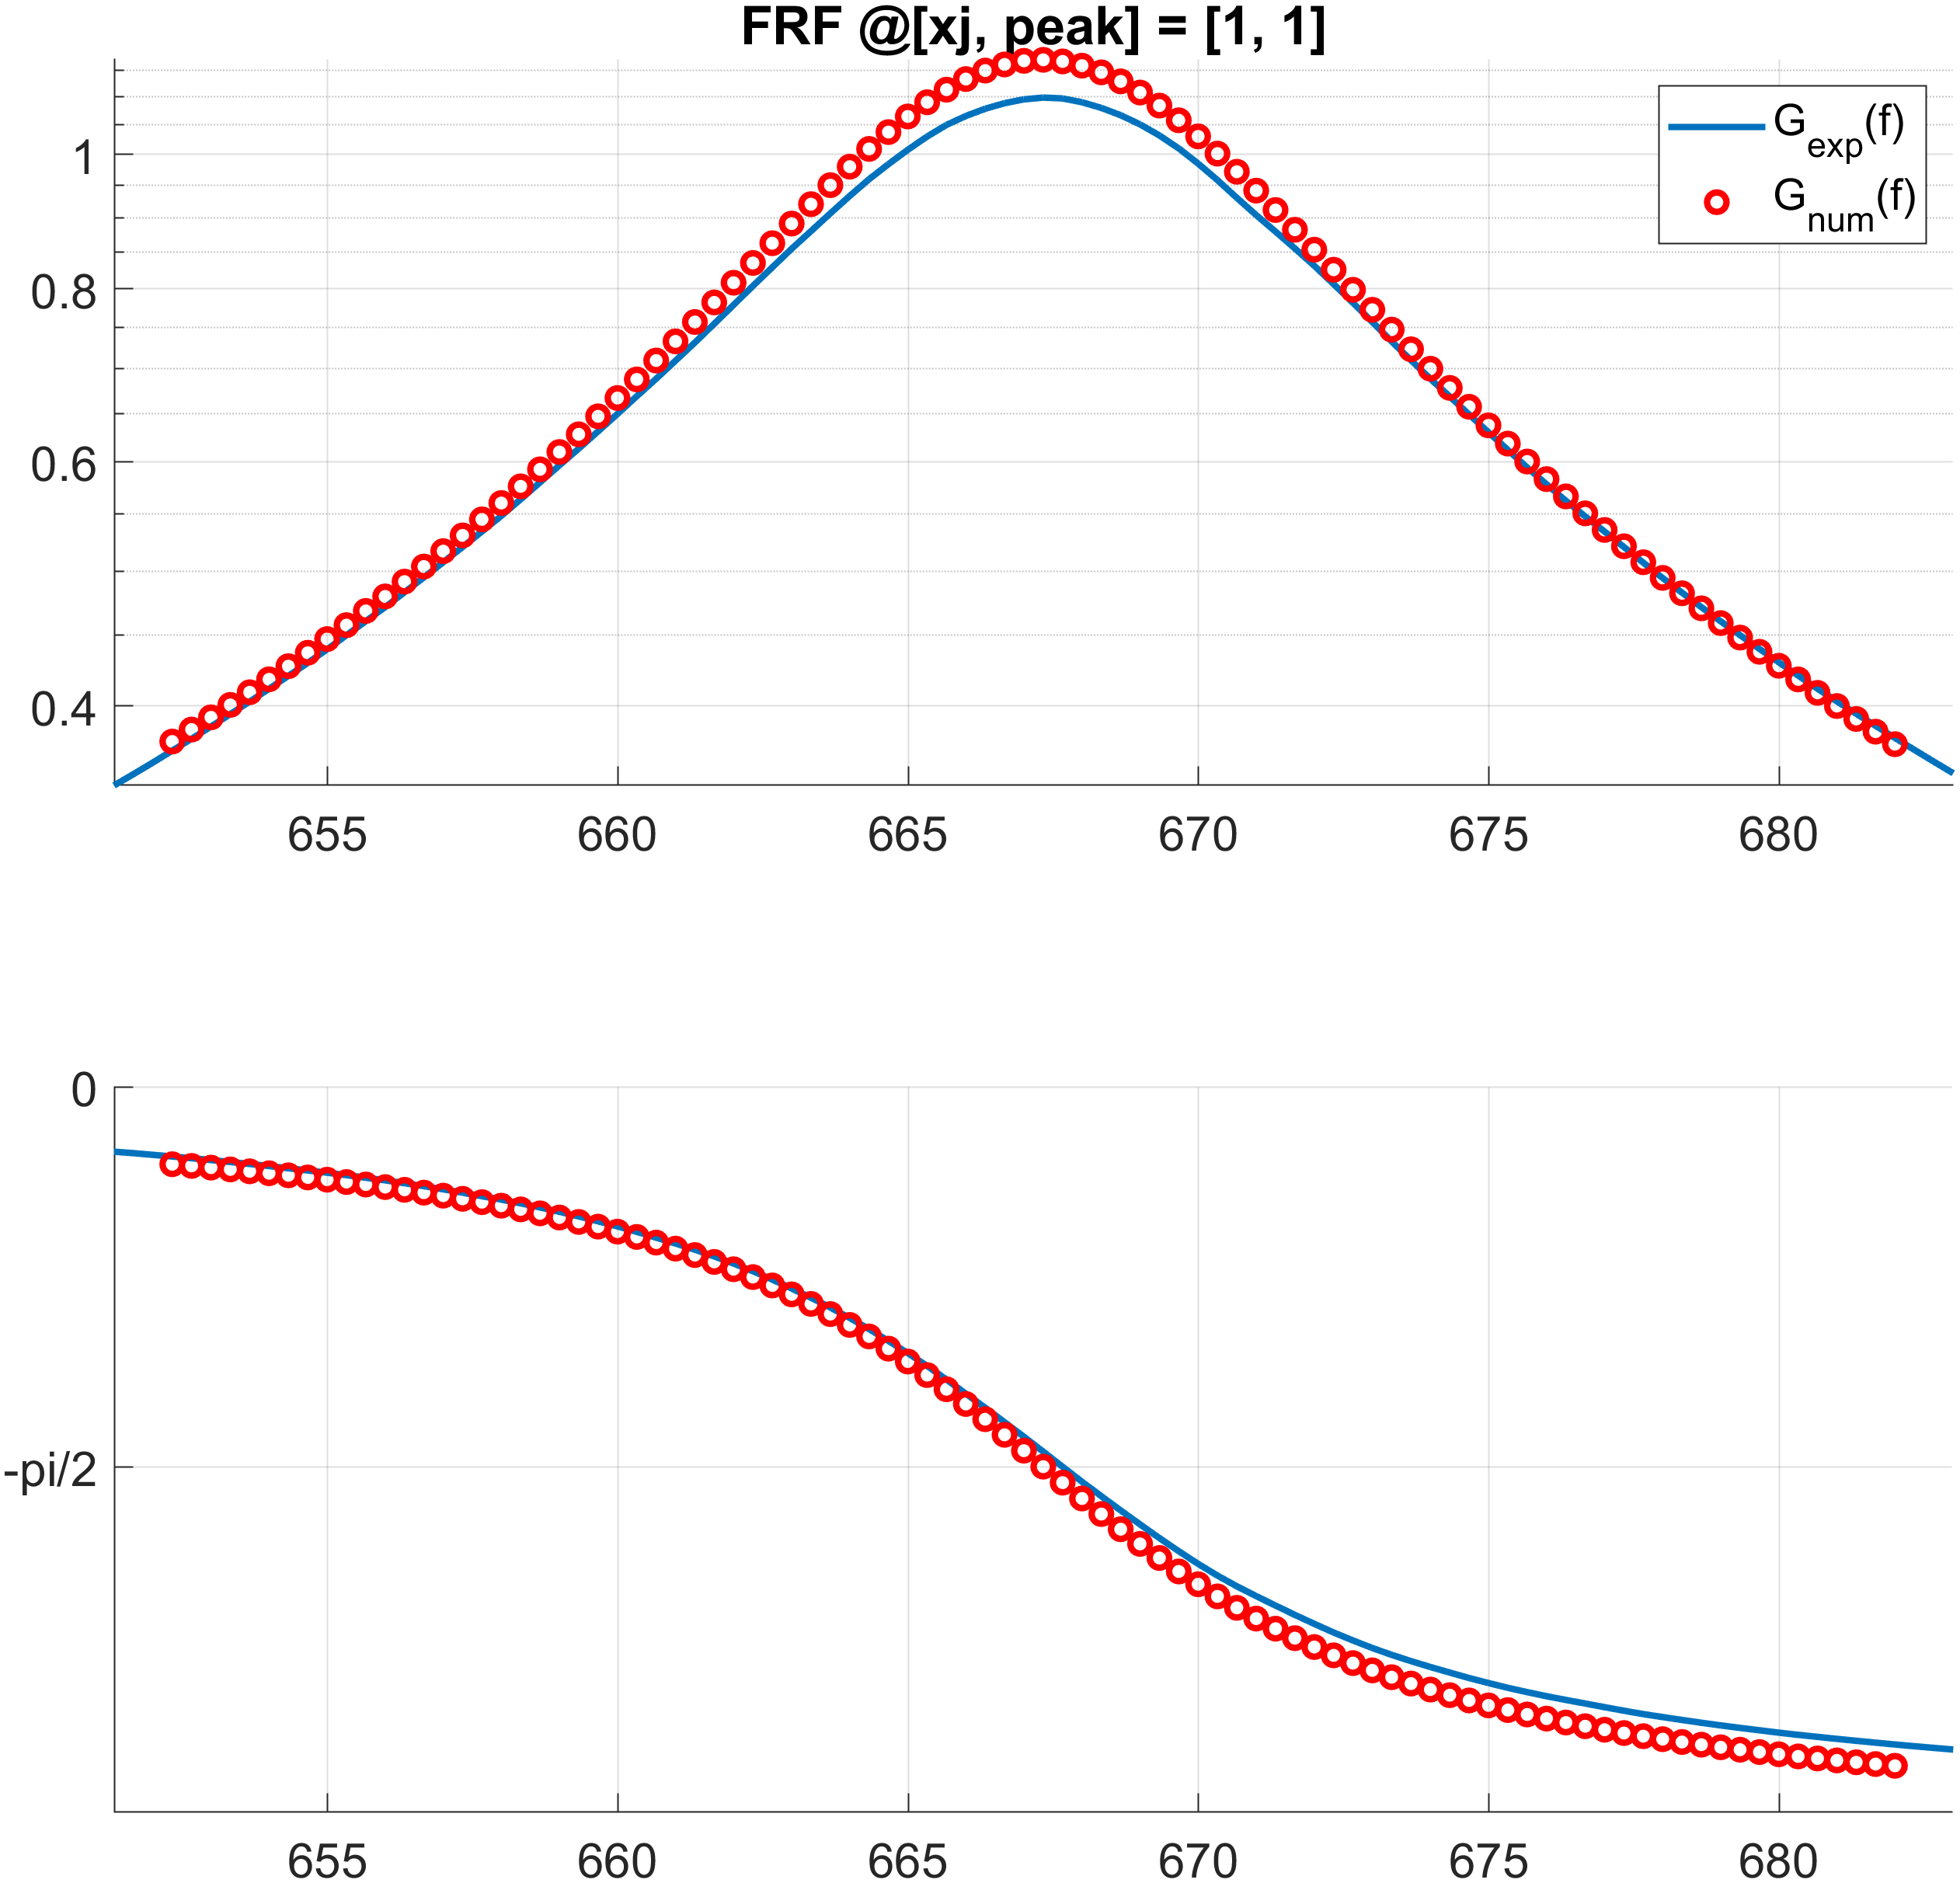
\includegraphics[width=0.6\textwidth]{img/MATLAB/Part_B/Comparison_FRF_1_zoom_peak_01.png}
    \caption{First peak FRFs comparison.}
    \label{fig:first_peak}
\end{figure}


